Teoria węzłów to gałąź topologii,
która powstała z~inspiracji węzłami,
jakie pojawiają się w~codziennym życiu: przy wiązaniu butów albo cumowaniu statków.
Zajmuje się ona badaniem przede wszystkim węzłów,
czyli pewnych włożeń okręgu $S^1$ w~trójwymiarową przestrzeń euklidesową $\R^3$ lub sferę $S^3$,
ale także splotów (zaplątanych w~sobie węzłów), warkoczy, supłów oraz podobnych obiektów.
Matematyczne węzły różnią się tym od zwykłych, że ich końce są ze sobą połączone.

Oto kilka przykładów.
Węzeł (a) nazywamy niewęzłem (jest to kalka angielskiego \emph{unknot}).
Następne w~kolejce widoczne są trójlistnik (b,~\emph{trefoil}), ósemka (c,~\emph{figure-eight}), pięciolistnik (d,~\emph{cinquefoil}) oraz słynna para Perko (e,~f~wg oryginalnej numeracji Rolfsena).

\begin{figure}[H]
	\centering
	\begin{minipage}[b]{.14\linewidth}
		\centering
		$\begin{tikzpicture}[baseline=-0.65ex, scale=0.5] \begin{knot}[clip width=5, end tolerance=1pt] \strand[semithick] (0,0) circle (\linewidth); \end{knot}
\end{tikzpicture}$
		\subcaption{}
	\end{minipage}
	\begin{minipage}[b]{.14\linewidth}
		\centering
		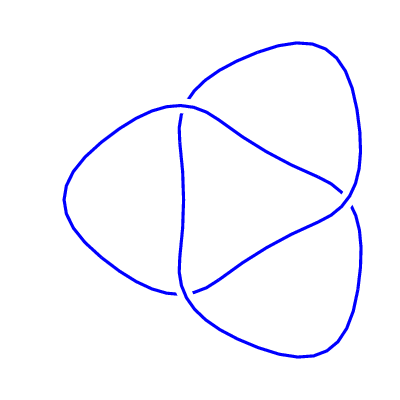
\includegraphics[width=\linewidth]{../data/3_1.png}
		\subcaption{$3_1$}
	\end{minipage}
	\begin{minipage}[b]{.14\linewidth}
		\centering
		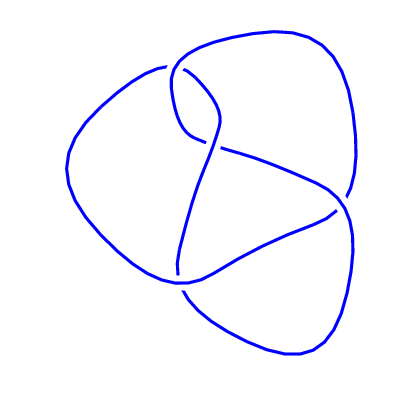
\includegraphics[width=\linewidth]{../data/4_1.png}
		\subcaption{$4_1$}
	\end{minipage}
	\begin{minipage}[b]{.14\linewidth}
		\centering
		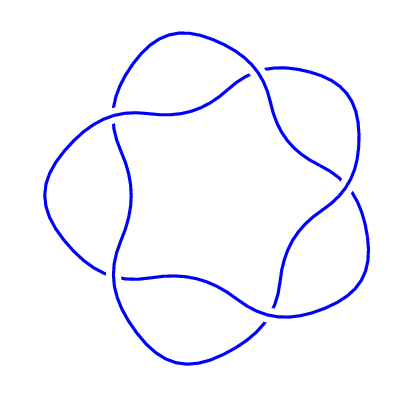
\includegraphics[width=\linewidth]{../data/5_1.png}
		\subcaption{$5_1$}
	\end{minipage}
	\begin{minipage}[b]{.14\linewidth}
		\centering
		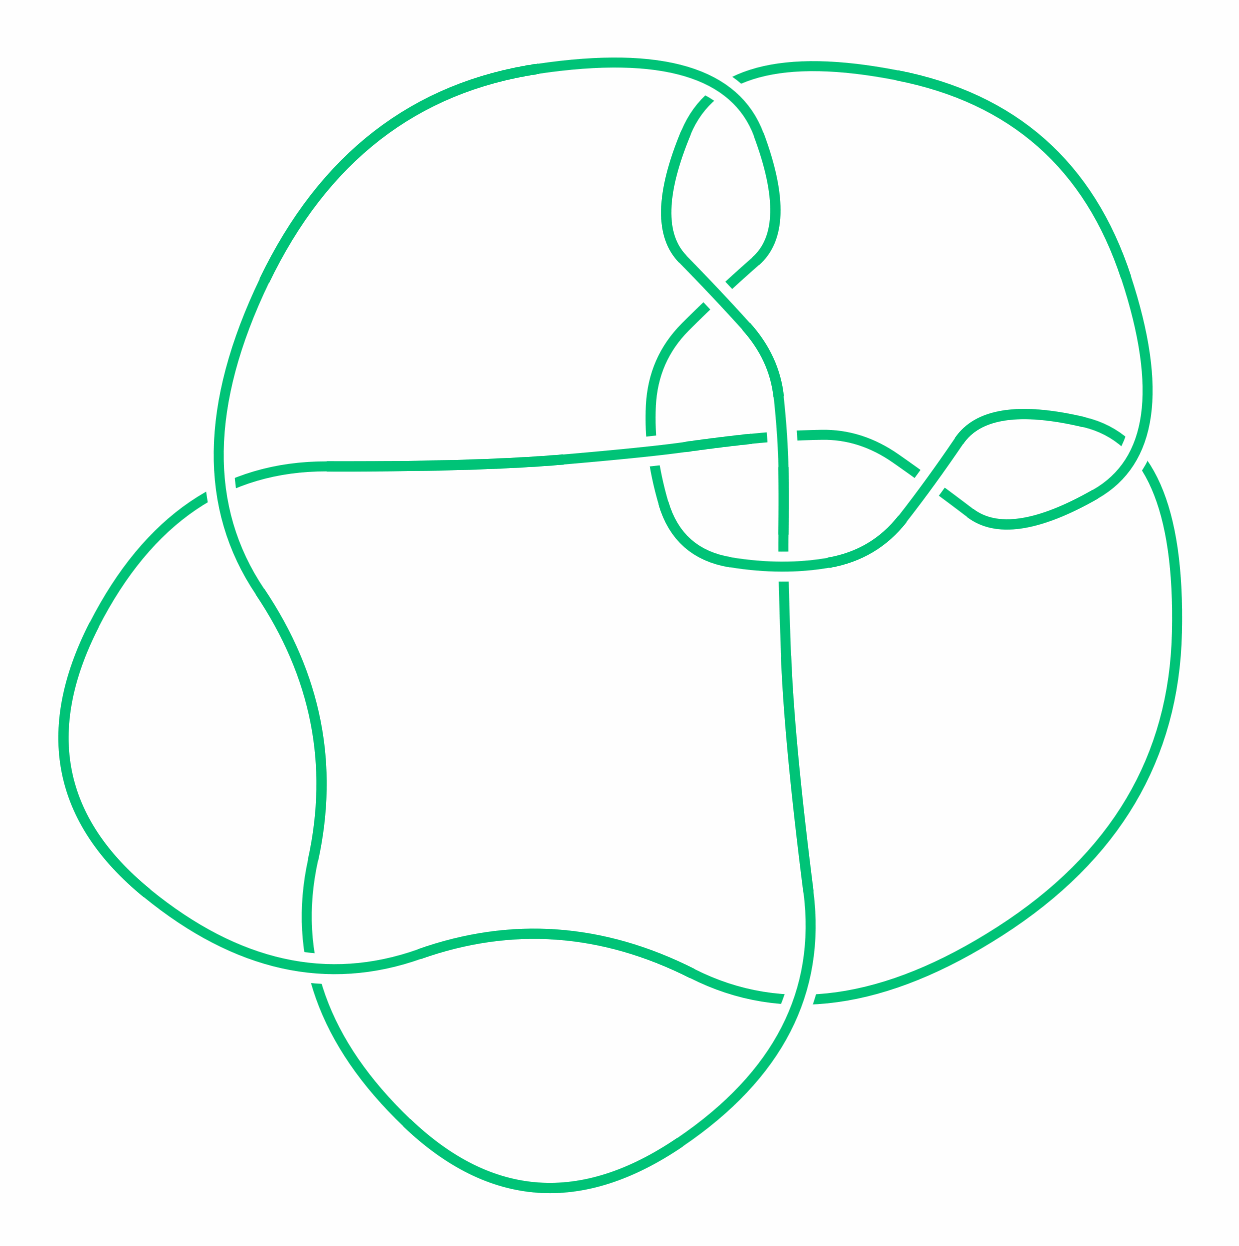
\includegraphics[width=\linewidth]{../data/perko1.png}
		\subcaption{$10_{161}$}
	\end{minipage}
	\begin{minipage}[b]{.14\linewidth}
		\centering
		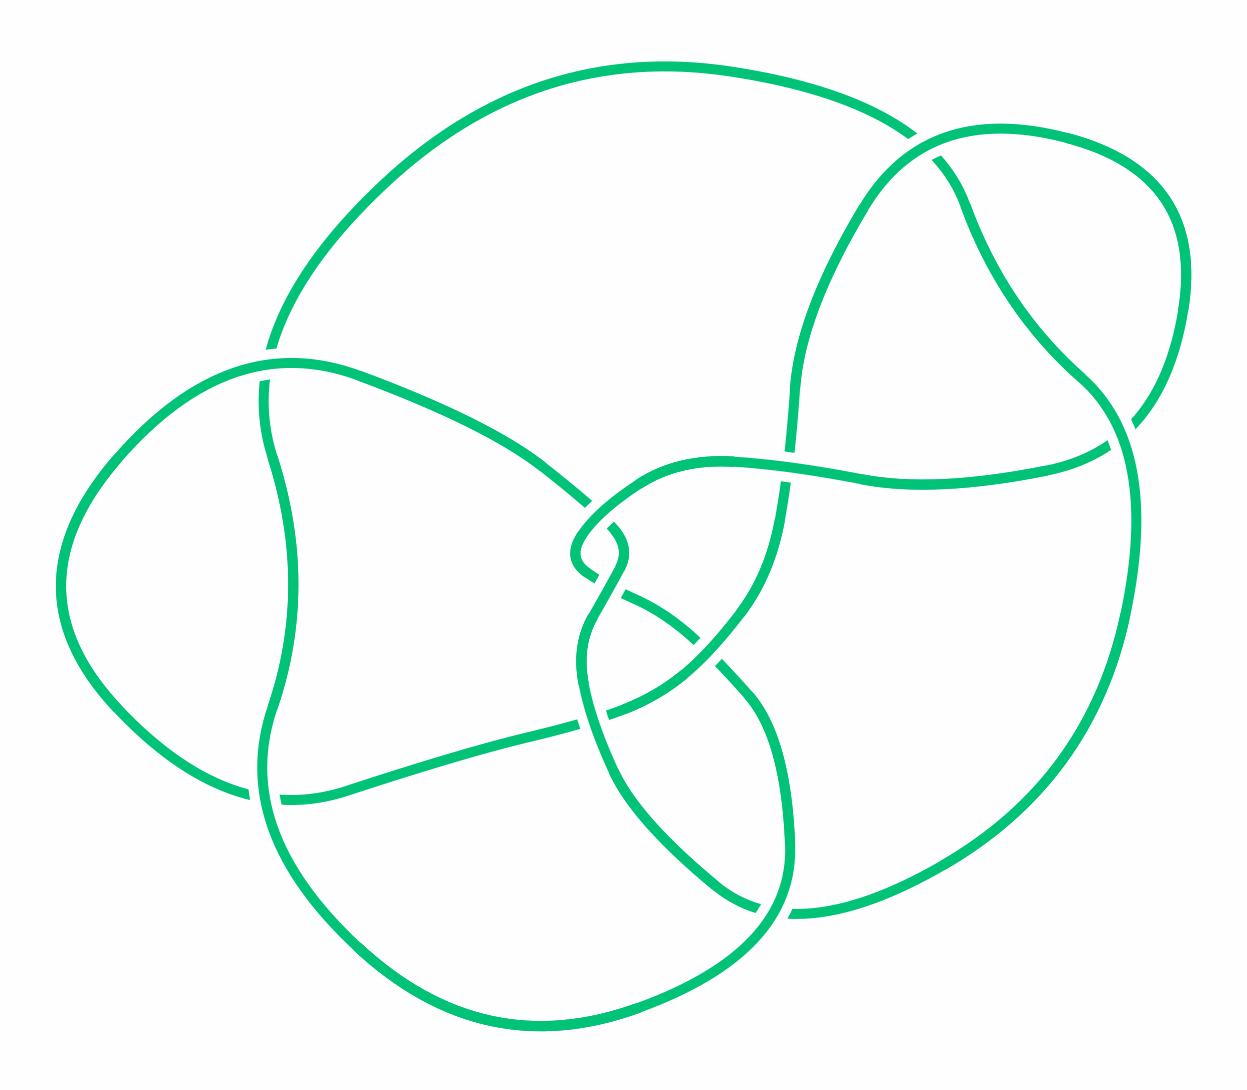
\includegraphics[width=\linewidth]{../data/perko2.png}
		\subcaption{$10_{162}$}
	\end{minipage}
\end{figure}

Początkowo celem teorii węzłów była klasyfikacja wszystkich węzłów.
Od XIX wieku, kiedy teoria węzłów wyodrębniła się jako osobny dział matematyki,
zdążyliśmy skatalogować ponad sześć miliardów tych obiektów.
Pozornie tak samo wyglądające węzły mogą się od siebie różnić.
Do wykrywania tych subtelnych różnic używa się przede wszystkim niezmienników topologicznych takich jak grupy, wielomiany bądź liczby.
Poznamy je w~dalszych rozdziałach.

Matematycy uogólnili pojęcie węzła:
można rozpatrywać je w~wyższych wymiarach albo zastąpić okrąg inną przestrzenią topologiczną.
Będziemy starać się unikać tych uogólnień.

\section{Węzły i~sploty}
Największą różnicą między węzłami matematycznymi oraz tymi z~prawdziwego jest życia jest to, że te pierwsze nie mają luźnych końców.
Można przyjąć nieidealną, naiwną definicję:

\begin{definition}
	Ciągłe oraz różnowartościowe odwzorowanie $S^1 \to \R^3$ to \textbf{węzeł}.
\end{definition}

Zastanówmy się, jakim formalizmem opisać manipulowanie fizycznym sznurkiem.
Nie można użyć izotopii
(dwa węzły są izotopijne, jeśli istnieje ciągła funkcja $F \colon S^1 \times [0, 1] \to \R^3$ taka, że $F(-, 0)$ jest pierwszym, zaś $F(-,1)$ drugim węzłem).
Zauważmy, że każde splątanie ściąga się do punktu.
Dowolny węzeł jest równoważny z~trywialnym, zatem istnieje tylko jedna klasa abstrakcji.
\begin{figure}[H]
	\begin{minipage}[b]{.23\linewidth}
		\centering
		
\includegraphics[width=\linewidth]{../data/missing.jpg}
		\subcaption{węzeł}
	\end{minipage}
	\begin{minipage}[b]{.23\linewidth}
		\centering
		
\includegraphics[width=\linewidth]{../data/missing.jpg}
		\subcaption{prostszy węzeł}
	\end{minipage}
	\begin{minipage}[b]{.23\linewidth}
		\centering
		
\includegraphics[width=\linewidth]{../data/missing.jpg}
		\subcaption{niewęzeł}
	\end{minipage}
\end{figure}

Trzeba uwzględnić to, jak węzeł leży w~przestrzeni.
Właściwym narzędziem jest więc izotopia otaczająca.
Intuicyjnie: dwa węzły uznajemy za równoważne,
jeśli można przejść od jednego do drugiego przy użyciu deformacji całej przestrzeni $\R^3$.

\begin{definition}[izotopia otaczająca] \label{def_ambient_isotopy}
	Ciągłe odwzorowanie $F \colon \R^3 \times [0,1] \to \R^3$,
	które staje się homeomorfizmem po ustaleniu drugiego argumentu i~takie,
	że $F(-, 0)$ jest funkcją tożsamościową,
	zaś $F(-, 1)$ złożona z~pierwszym węzłem daje drugi węzeł,
	nazywamy izotopią otaczającą.
\end{definition}

\begin{definition}[węzeł]
	\label{def:knot}
	\index{węzeł}
	Gładkie włożenie $S^1 \to \R^3$ izotopijne otaczająco z~zamkniętą łamaną bez samoprzecięć nazywamy węzłem poskromionym.
\end{definition}

Wykluczamy w~ten sposób patologiczne z~kombinatorycznego punktu widzenia węzły dzikie.
Przez prawie całą książkę interesować nas będą jedynie węzły poskromione,
dlatego jeśli nie zaznaczono inaczej, przez węzeł rozumiemy węzeł poskromiony.
\todo{Wstawić przykład węzła dzikiego.}
Dość często będziemy utożsamiać węzeł z~jego obrazem.

Jednocześnie homeomorfizmy $F(-,t)$ zastępujemy przez dyfeomorfizmy zachowujące orientację.
Chwila namysłu wystarcza do przekonania się, że definicja \ref{def_ambient_isotopy} obejmuje zwykłą izotopię,
a przy tym nie pozwala na rozwiązanie nietrywialnych węzłów przez ściągnięcie zaplątania do punktu.
Istnieje jeszcze jedna, konkurencyjna definicja węzłów równoważnych:

\begin{definition}
	Dwa węzły są równoważne, gdy jeden z~nich jest obrazem drugiego przez zachowujący orientację homeomorfizm $\R^3 \to \R^3$.
\end{definition}

Stwierdzenie to przestaje być prawdziwe po zastąpieniu przestrzeni $\R^m$ przez $S^m$.

\begin{proof}
	Podany niżej dowód pochodzi z~książki ,,Topology from the differentiable viewpoint'' Johna Milnora.
	Musimy pokazać, że dyfeomorfizm $f \colon \R^m \to \R^m$ jest gładko izotopijny z~identycznością.
	Translacje są izotopiami, więc bez straty ogólności zakładamy, że $f(0) = 0$.
	Pochodna $f$ w~zerze jest dana wzorem $\mathrm{d}f_0(x) = \lim_{t \to 0} f(tx) /t$,
	naturalną definicją	izotopii $F \colon \R^m \times [0, 1] \to \R^m$ jest więc
	\[
		F(x, t) = \begin{cases}
			f(tx) / t & 0 < t \le 1 \\
			\mathrm{d}f_0(x) & t = 0
		\end{cases} .
	\]

	Funkcja $F$ jest gładka,
	gdyż na mocy lematu Hadamarda funkcja $f$ zapisuje się jako suma $x_1 g_1(x) + \ldots + x_mg_m(x)$,
	gdzie funkcje $g_i$ są gładkie, co jakoś kończy dowód.
\end{proof}

\begin{definition}[splot]
	\label{def_link}
	\index{splot}
	Sumę rozłączną skończenie wielu węzłów nazywamy splotem.
\end{definition}

\begin{example}
	\index{splot!Hopfa}
	Whitehead w~1934 odkrył kontrprzykład do nieudanego dowodu hipotezy Poincarego.
	Był nim splot o~dwóch składowych przedstawiony na poniższym rysunku.
	Splot Hopfa to najprostszy splot nietrywialny, którym w~1931 r. zajmował się Heinz Hopf,
	topolog niemiecki, w~ramach badań nad tzw. rozwłóknieniem (Hopf fibration).

	\begin{figure}[H]
		\begin{minipage}[b]{.32\linewidth}
			\centering
			
\includegraphics[width=\linewidth]{../data/missing.jpg}
			\subcaption{splot Whiteheada}
		\end{minipage}
		\begin{minipage}[b]{.32\linewidth}
			\centering
			
\includegraphics[width=\linewidth]{../data/missing.jpg}
			\subcaption{splot Heada}
		\end{minipage}
		\begin{minipage}[b]{.32\linewidth}
			\centering
			
\includegraphics[width=\linewidth]{../data/missing.jpg}
			\subcaption{splot jakiś inny}
		\end{minipage}
	\end{figure}
\end{example}

\begin{definition}[rozszczepialność]
	\index{splot!rozszczepialny}
	Splot, który jest niespójną sumą niepustych splotów, nazywamy rozszczepialnym.
\end{definition}

Jeśli dwa węzły są równoważne, to ich dopełnienia są oczywiście homeomorficzne.
Pytanie o~prawdziwość implikacji odwrotnej jako pierwszy zadał najprawdopodobniej Tietze\footnote{Praca \emph{Über die topologischen Invarianten mehrdimensionaler Mannigfaltigkeiten}.} w~1908 roku.
Od 1989 roku znamy odpowiedź na nie, jest pozytywna: każdy węzeł jest wyznaczony jednoznacznie przez swoje dopełnienie.
Wcześniej pokazano, że istnieją co najwyżej dwa węzły o~zadanym dopełnieniu.

\begin{theorem}[Gordon, Luecke, 1989] \label{thm_gordon_luecke}
	\index{twierdzenie!Gordona-Lueckego}
	Poskromione węzły o~homeomorficznych (z zachowaniem orientacji) dopełnieniach są wzajemnie izotopijne.
\end{theorem}

Twierdzenie to zamienia problem lokalny (czy dwa węzły w kuli $S^3$ są równoważne?) w~problem globalny (czy dwie przestrzenie topologiczne są homeomorficzne?).

\begin{proof}[Niedowód]
	Wynika to z~ogólniejszego stwierdzenia:
	nietrywialna chirurgia Dehna na węźle w~3-sferze nigdy nie daje 3-sfery.
	Pełny dowód zawiera praca \cite{gordon89}.
\end{proof}

Istnieje nieskończenie wiele (jakich?) kontrprzykładów do odpowiednika twierdzenia Gordona-Lueckego dla splotów,
których nie da się, patrząc na samo dopełnienie, odróżnić od splotu Whiteheada.

\section{Diagramy}
Chociaż w~świetle definicji \ref{def:knot} węzły są pewnymi regularnymi podzbiorami przestrzeni $\R^3$,
z kombinatorycznego punktu widzenia wygodniej jest rysować je na  płaszczyźnie.

\begin{definition} [diagram] \label{def_diagrams}
	\index{diagram}
	Cień to rzut węzła $K \subseteq \R^3$ na płaszczyznę.
	Diagram to cień bez katastrof
	(potrójnych przecięć, stycznych i~dziobów)
	razem z~informacją o~tym, jak przebiegają skrzyżowania.
\end{definition}

\begin{definition} [włókno]
	\index{włókno}
	Fragment diagramu, który biegnie między dwoma kolejnymi tunelami (podskrzyżowaniami) nazywamy włóknem.
\end{definition}

\begin{proposition}
	Każdy splot posiada diagram -- zbiór diagramów jest otwarty i~gęsty w~zbiorze wszystkich.
\end{proposition}

\begin{proof}
	Rzut splotu na równoległe płaszczyzny jest taki sam,
	a te można sparametryzować prostymi przechodzącymi przez początek układu współrzędnych,
	które tworzą przestrzeń rzutową $\R \mathbb P^2$.
	Niech $S$ będzie zbiorem prostych, które dają złe rzuty.
	Wystarczy pokazać jego nigdziegęstość.
	Okazuje się, że $S$ jest też jednowymiarowy.
	(Dowód za \cite{crowell63}).
\end{proof}

\begin{definition}
	\index{węzeł!alternujący}
	Diagram jest alternujący,
	gdy podczas poruszania się wzdłuż splotu
	mijamy jego skrzyżowania na zmianę z~góry oraz z~dołu.
	Splot jest alternujący, gdy posiada taki diagram.
\end{definition}

%Niestety pomimo upływu czasus, nikt nie napisał komputerowego programu realizującego ten algorytm (stan na 1994).
%Może podejmie się tego Czytelnik?
%Inne algorytmy istnieją, jednak wszystkie działają w~wykładniczym czasie.

W 1961 roku W. Haken \cite{haken61} podał niezawodny przepis na wykrycie diagramu niewęzła,
częściowo rozwiązując jeden z~ważniejszych problemów teorii węzłów.
Przez wiele lat nikt nie podjął się implementacji tego algorytmu,
udało się to na przykład B. Burtonowi, R. Budneyowi oraz W. Petterssonowi w~komputerowym programie Regina
\footnote{Dostępny pod adresem \url{https://regina-normal.github.io/}.} na przełomie tysiącleci.
Burton, Rubinstein i~Tillman pokazali w~pracy \cite{burton12}, jak sprawdzać,
czy powierzchnia normalna na striangulowanej 3-rozmaitości jest (nie)ściśliwa w~czasie wykładniczym.
To okazało się być wystarczającym do udzielenia negatywnej odpowiedzi na pytanie Thurstona:
,,czy przestrzeń Seiferta-Webera jest rozmaitością Hakena?'',
a zatem wykraczającego poza poziom tej pracy.
Patrz także {\url{http://geometrygames.org/SnapPea/index.html}.

Przykładami trudnych w~rozpoznaniu niewęzłów są: niewęzeł Goritza, Freedmana.

\begin{figure}[H]
	\begin{minipage}[b]{.32\linewidth}
		\centering
		
\includegraphics[width=\linewidth]{../data/missing.jpg}
		\subcaption{normalny}
	\end{minipage}
	\begin{minipage}[b]{.32\linewidth}
		\centering
		
\includegraphics[width=\linewidth]{../data/missing.jpg}
		\subcaption{Goritza}
	\end{minipage}
	\begin{minipage}[b]{.32\linewidth}
		\centering
		
\includegraphics[width=\linewidth]{../data/missing.jpg}
		\subcaption{Freedmana}
	\end{minipage}
\end{figure}

Więcej trudnych niewęzłów zawiera świeża praca
,,Algorithmic simplification of knot diagrams: new moves and experiments'
\footnote{\url{https://arxiv.org/pdf/1508.03226.pdf}}
C. Petronio, A. Zanellatiego.

Innym narzędziem wykrywającym niewęzły jest homologia Chowanowa (opisana później),
jak pokazał Kronheimer z~Mrówką \cite{kronheimer11}.
Bar-Natan, topolog izraelski, napisał program liczący te homologie szybko \cite{barnatan07},
zapewne w~czasie $O(\exp(c \sqrt n))$, dla diagramu o~$n$ skrzyżowaniach.
Nie możemy liczyć na istotne przyspieszenie:
znalezienie przybliżenia wielomianu Jonesa jest problemem \#P-trudnym (\cite{kuperberg15}, \cite{vertigan05}),
a przy znanych homologiach -- wręcz trywialnym.
Patrz też \ref{jones_sharp_p_hard}.

\subsection{Historia tablic węzłów}
Pierwszą osobą, która podjęła się szukania węzłów, był Peter Guthrie Tait, szkocki fizyk.
Razem z Thomsonem (lordem Kelvinem) wierzyli, że węzły są kluczem do zrozumienia widma spektroskopowego różnych pierwiastków: na przykład atom sodu mógł być splotem Hopfa ze względu na dwie linie emisyjne.
Eksperyment Michelsona-Morleya z 1887 roku zabił ich ,,wirową teorię atomu'', ale nie miało to znaczenia dla teorii węzłów jako działu matematyki.

Używana po dziś dzień strategia, którą przyjął Tait, jest stosunkowa prosta: narysować wszysktie możliwe diagramy o~zadanym indeksie skrzyżowaniowym, po czym połączyć ze sobą te, które przedstawiają jeden węzeł.
Na potrzeby pierwszego etapu Tait wymyślił schemat kodowania diagramów.
Wiele lat wcześniej, Gauss wraz ze swoim uczniem Listingiem badał węzły i~opracował (niezależnie!) podobną notację.
My przytoczymy opis dalszego ulepszenia tej metody, zwanego notacją Dowkera-Thistletwaite’a.

Tait wykorzystując swoją notację podał w~1876 pierwszą tablicę piętnastu węzłów o~mniej niż ośmiu skrzyżowaniach.
Nie należy traktować tego jako skromny wynik: nie miał on do dyspozycji żadnych twierdzeń topologicznych do odróżniania węzłów.
Onieśmielony przez liczbę możliwych ciągów dla kolejnych indeksów skrzyżowaniowych, powstrzymał się przed rozszerzaniem swojej tablicy.
To właśnie grupowanie diagramów przedstawiających ten sam węzeł, a~nie samo szukanie wszystkich możliwych diagramów, sprawia trudność.

Aby sobie pomóc, Tait znalazł lokalną modyfikację diagramu, która nie zmienia indeksu skrzyżowaniowego, znaną obecnie jako flype.

\todo[inline]{Narysować ruch flype.}

Inną taktykę szukania węzłów przyjał wielebny Thomas Kirkman: zaczynał od małego zbioru "nieredukowalnych" rzutów, do których systematycznie dokładał skrzyżowania.
Tait przeczytał pracę Kirkmana, po czym w~latach 1884/1885 opracował listę węzłów alternujących o~mniej niż 11 skrzyżowaniach.
Tuż przed oddaniem jej do druku odkrył inny spis węzłów stworzony przez amerykańskiego naukowca Charlesa Little'a.
Znalazł wtedy jeden duplikat u~siebie, natomiast u Little'a jeden duplikat i~jedno pominięcie.

Zachęcony przez Taita, Little zabrał się za alternujące węzły o~11 skrzyżowaniach i~za trudniejsze zadanie, stablicowanie węzłów niealternujących, czyli takich, które nie posiadają alternującego diagramu.
Jak wynika z~pierwszej pracy Taita, początkowo nie wierzono, że takie w~ogóle istnieją.
Dowód znaleziono dopiero w~1930 roku, niealternujące są $8_{19}$, $8_{20}$, $8_{21}$, ale nie węzły o mniejszej liczbie skrzyżowań.
Little pracował przez sześć lat (1893 -- 1899) i~znalazł 43 niealternujące węzły o~10 skrzyżowaniach.
Żadnego nie pominął, ale trafił mu się jeden duplikat.
Sundberg, Thistlethwaite pokazali w 1998 roku, że stosunek liczby splotów alternujących do wszystkich maleje wykładniczo (\cite{sundberg98}):

\begin{proposition}
    Niech $a_n$ oznacza liczbę pierwszych, alternujących supłów o $n$ skrzyżowaniach.
    Wtedy $a_n \sim (3c_1/4\sqrt{\pi})n^{-5/2}\lambda^{n-3/2}$, gdzie $c_1$ i $\lambda = (101 + \sqrt{21001})/40$ są jawnie znanymi stałymi.
    Niech $A_n$ oznacza liczbę pierwszych, alternujących splotów o $n$ skrzyżowaniach.
    Wtedy $A_n \approx \lambda^n$, dokładniej: jeśli $n \ge 3$, to
    \[
    	\frac{a_{n-1}}{16n - 24} \le A \le \frac{a_n - 1}{2}.
    \]
\end{proposition}

W kolejnych dziesięcioleciach nie nastąpił znaczący postęp, zarówno w~rozszerzaniu tablic jak i~sprawdzaniu tych już istniejących.
Haseman w~1918 roku znalazł achiralne węzły o~12 i~14 skrzyżowaniach.
W 1927 roku Alexander z~Briggsem przy użyciu pierwszej grupy homologii rozgałęzionego nakrycia cyklicznego (!) potrafili odróżnić od siebie dowolne dwa węzły (z~pominięciem trzech par) o~co najwyżej 9 skrzyżowaniach.
Reidemeister poradził sobie z~tymi wyjątkami w~1932 roku, korzystając z~indeksu zaczepienia i~homomorfizmów z~grupy węzła na grupy diedralne.
% branch curves in irregular covers associated to homomorphisms of the knot group onto dihedral groups

%%%%% Tait, Little wyprodukowali prawie bezbłędną tablicę węzłów o~co najwyżej 11 skrzyżowaniach przy użyciu grafów.

Dopiero Conway w~latach sześćdziesiątych minionego wieku znalazł pierwsze węzły o~mniej niż 12 skrzyżowaniach oraz wszystkie sploty o~mniej niż 11 skrzyżowaniach w~oparciu o~pomysły Kirkmana.
% An enumeration of knots and links, 1970.
Zajęło mu to jedynie kilka godzin!
Conway znalazł 1 duplikat oraz 11 pominięć w~tablicach Little'a, ale sam popełnił 4 pominięcia.
Przeoczył między innymi słynny duplikat w~niealternującej tablicy Little'a, parę Perko.
% 1974?
Przyczyną było prawdopodobnie to, że dwa diagramy miały różny spin:
Little błędnie twierdził, że spin minimalnego diagramu jest niezmiennikiem, gdyż błędnie założył, że flype oraz 2-przejścia wystarczają do zmiany jednego minimalnego diagramu w~inny.

Pominęcia w~tablicy Conwaya znalazł Caudron w~1980 roku.
Nieopublikowany manuskrypt Bonahona, Siebenmanna klasyfikuje węzły algebraiczne.
Z~nielicznymi niealgebraicznymi węzłami do 11 skrzyżowań poradził sobie Perko około 1980 roku (,,Invariants of 11-crossing knots'').
To był kres ery ręcznych obliczeń.

Na początku lat osiemdziesiątych Dowker i~Thistlethwaite stabularyzowali z~pomocą komputera węzły do 13 skrzyżowań.
Przez blisko dekadę nic się nie działo, aż grupa studentów wygrała dostęp do superkomputera Cray.
Razem z~Hoste znaleźli alternujące węzły do 14 skrzyżowań, jednocześnie sprawdzając istniejące tabele Thistlethwaite'a.
Około roku 1998 Hoste z~Weeksem (oraz niezależnie Thistlethwaite) znaleźli 1701936 pierwszych węzłów do 16 skrzyżowań.
Spośród nich, tylko 32 nie jest węzłami hiperbolicznymi, wszystkie pozostałe poddają się maszynerii geometrii hiperbolicznej.

\subsection{Hipotezy Taita}
\begin{conjecture}[I hipoteza Taita]
	\label{conj_tait_i}
	\index{hipoteza!Taita}
	Zredukowany alternujący diagram (splotu) ma minimalny indeks skrzyżowaniowy.
\end{conjecture}
% To bardzo ważny rezultat, którego prawdziwość przypuszczał już P. G. Tait w~XIX wieku.
% Nikt nie był w~stanie podać dowodu przed pojawieniem się wielomianu Jonesa.

\begin{conjecture}[II hipoteza Taita]
	\label{conj_tait_ii}
	Achiralny splot alternujący ma zerowy spin.
\end{conjecture}

\begin{conjecture}[III hipoteza Taita]
	\label{conj_tait_iii}
	Niech $D_1, D_2$ będą zredukowanymi alternującymi diagramami zorientowanego pierwszego splotu.
	Wtedy diagram $D_2$ można otrzymać z~$D_1$ korzystając jedynie z~ruchu \emph{flype}.
\end{conjecture}

Z III hipotezy Taita wynika, że dwa zredukowane diagramy alternujące tego samego węzła mają ten sam spin: ruch flype nie zmienia spinu.
Bezpośredni dowód przeprowadzili Murasugi (1987) i Thistlethwaite (1988).
My pokażemy nieco później, czyli po poznaniu wielomianu Jonesa, że wszystkie trzy hipotezy są prawdziwe.

\subsection{Metody kodowania}
\subsubsection{Notacja Dowkera--Thistlethwaite'a}
Poprawia notację Taita.
Przypisuje ona (niejednocznacznie) każdemu węzłowi permutację znakowanych liczb parzystych $\pm 2, \pm 4, \ldots, \pm 2N$.

\subsubsection{Notacja Alexandera-Briggsa}
Najbardziej tradycyjna, wprowadzona w~1927 roku, rozszerzona później przez Rolfsena.

\subsubsection{Notacja Conwaya}
Wprowadzona przez Conwaya w~pracy ,,An Enumeration of Knots and Links, and Some of Their Algebraic Properties''.

% A pictorial enumeration of prime knots of up to 10 crossings appears in Rolfsen (1976, Appendix C).
% Note, however, that in this table, the Perko pair 10-161 and 10-162 are actually identical, and the uppermost crossing in 10-144 should be changed (Jones 1987).

% Rolfsen's last four 10 crossing knots have been renumbered, to avoid the Perko duplication.
% A further mistake in Rolfsen's tables is that therein 1083 and 1086 were swopped: the Conway notation and Alexander polynomial for each one referred to the diagram of the other.
% We exchange not diagrams, but Alexander polynomial and Conway notation to fix the mistake (like the table in the new 2003 edition of the Rolfsen book, Dror Bar-Natan's Knot Atlas, and Chuck Livingston's Table of Knot Invariants, and unlike in Kawauchi's book!).
% http://stoimenov.net/stoimeno/homepage/ptab/
